\chapter{TINJAUAN PUSTAKA}
\label{chap:tinjauanpustaka}

% Ubah bagian-bagian berikut dengan isi dari tinjauan pustaka
Demi mendukung penelitian ini, dibutuhkan beberapa teori penunjang sebagai bahan acuan dan referensi. Dengan demikian penelitian ini menjadi lebih terarah.

\section{Berita Palsu}
\label{sec:beritapalsu}

Berita palsu atau biasa dikenal dengan berita hoaks adalah sebuah informasi yang sesungguhnya tidak benar, tetapi dibuat seolah - olah benar adanya \cite{berita_bohong}. Di Indonesia sendiri, hoaks menjadi sebuah masalah tersendiri, hal ini karena masih banyak masyarakat yang langsung mempercayai apapun yang mereka temui di internet tanpa melakukan cek fakta terlebih dahulu.

Ada banyak sekali efek dari berita palsu ini, mulai dari hilangnya reputasi sampai nyawa yang terancam. Salah satu contoh kasus yang cukup parah adalah kerusuhan yang terjadi di Papua, dimana kerusuhan tersebut disebabkan karena adanya hoaks soal ucapan rasialis dari seorang guru SMP kepada muridnya \cite{efek_hoax}.

\section{\textit{Machine Learning}}

\textit{Machine Learning} atau Pembelajaran Mesin adalah salah satu cabang dalam kecerdasan buatan dan ilmu komputer yang menggunakan data dan algoritma untuk meniru manusia dalam mempelajari sesuatu \cite{ibm_ml_expl}. Salah satu hal yang membuat pembelajaran mesin sangat diminati adalah kemampuannya untuk menyelesaikan suatu tugas dengan sedikit intervensi dari manusia.

Sekarang ini, pembelajaran mesin adalah salah satu fokus yang cukup diminati pada bidang \textit{data science}. Dimana dengan menggunakan pembelajaran mesin, diharapkan suatu kecerdasan buatan dapat menyelesaikan beberapa tugas yang bagi komputer cukup rumit seperti misalnya, memberikan prediksi yang akurat berdasarkan data, melakukan klasifikasi pada teks maupun pada gambar, melakukan pemrosesan citra guna mengenali objek di dalam citra tersebut, dan masih banyak lagi.

Untuk prosesnya sendiri, awalnya kita harus mengumpulkan data, data ini dapat kita ambil dari  berbagai sumber atau bisa juga menggunakan data yang berasal dari instansi atau pribadi (data yang kita buat sendiri). Selanjutnya adalah proses \textit{training} dimana data akan dimasukkan ke dalam model pembelajaran mesin yang sudah dipilih. Kita dapat merubah beberapa parameter dari model tersebut untuk meningkatkan akurasi dari suatu model pembelajaran mesin. Terakhir adalah melakukan proses \textit{testing}, dimana model akan melakukan prediksi pada set data yang berbeda dari yang digunakan pada saat proses \textit{training}. Apabila ternyata tingkat akurasi dirasa kurang memadai, dapat dilakukan proses \textit{re-training} sampai tingkat akurasi nya dirasa cukup. Hasil akhir dari proses ini adalah sebuah model pembelajaran mesin yang dapat digunakan walaupun menggunakan data yang berbeda \cite{mit_ml_expl}.

\subsection{\textit{Supervised Learning}}

Salah satu cabang dalam bidang pembelajaran mesin. Disini data yang dijadikan masukan ke model sudah diberikan label atau struktur tertentu \cite{ms_ml_expl}. Berdasarkan dari data berlabel tersebut, sebuah model akan merubah parameter internalnya agar mendekati atau sesuai dengan label yang diberikan \cite{ibm_ml_expl}. Salah satu contoh model pembelajaran mesin dengan metode pembelajaran seperti ini adalah \textit{Linear Regression, Random Forest}, dan sebagainya.

\subsection{\textit{Unsupervised Learning}}

Salah satu cabang dalam bidang pembelajaran mesin. Disini data yang dijadikan masukan ke model tidak diberikan label sama sekali. Nantinya model akan membuat pengelompokan (\textit{clusters}) dan hubungan berdasarkan dari data yang diberikan \cite{mit_ml_expl}. Contoh model yang menggunakan metode pembelajaran ini adalah \textit{BERT, GPT-2/3} dan sebagainya.

\subsection{\textit{Reinforcement Learning}}

Salah satu cabang dalam bidang pembelajaran mesin. Disini model tidak diberikan data awal sama sekali, namun, model dibiarkan melakukan proses percobaan secara mandiri terus-menerus sampai tercapai hasil atau respon yang diinginkan. Apabila terdapat parameter yang menghasilkan respon positif, maka parameter tersebut disimpan dan digunakan sebagai masukan untuk iterasi \textit{training} berikutnya \cite{mit_ml_expl}.

\section{\textit{Deep Learning}}

Mirip seperti pembelajaran mesin, \textit{Deep Learning} juga merupakan salah satu bidang dalam bidang kecerdasan buatan. Yang membedakan antara pembelajaran mesin biasa dengan \textit{deep learning} adalah penggunaan \textit{layer} yang sangat banyak dibandingkan dengan pembelajaran mesin yang hanya memiliki 3 \textit{layers}. Keuntungan dari model jenis ini adalah model ini dapat memproses masukan yang paling abstrak sekalipun, sehingga menghilangkan proses ekstraksi fitur secara manual \cite{mathwork_deeplearning}. Namun, karena \textit{deep learning} memiliki \textit{layers} yang sangat banyak, maka diperlukan jumlah data yang jauh lebih banyak pula, karena itu pulalah, sebuah model \textit{deep learning} memerlukan daya komputasi yang jauh lebih besar dibandingkan dengan model pembelajaran mesin biasa \cite{mit_ml_expl}.

Gambar \ref{fig: deeplearning_layer} merupakan contoh bentuk \textit{layer} dalam suatu model \textit{deep learning} yang menggunakan 4 \textit{layers} didalamnya. Setiap \textit{layer} dapat memiliki fungsi dan tanggung jawabnya masing - masing \cite{mit_ml_expl}, seperti misal apabila kita menggunakan \textit{deep learning} untuk mendeteksi angka plat nomor di kendaraan bermotor, bisa saja beberapa layer pertama berfungsi untuk mendeteksi letak plat nomor dalam suatu citra, kemudian beberapa layer selanjutnya berfungsi untuk mengambil bentuk dari setiap objek dalam plat nomor tersebut, beberapa layer terakhir berfungsi untuk mengenali bentuk - bentuk dari objek menjadi tulisan teks. Semakin banyak layer yang digunakan, maka semakin tinggi pula kemungkinan kita melakukan sesuatu yang lebih kompleks \cite{mit_ml_expl}.

\begin{figure}[ht]
    \centering
    % Ubah file gambar berikut dengan file foto dari mahasiswa
    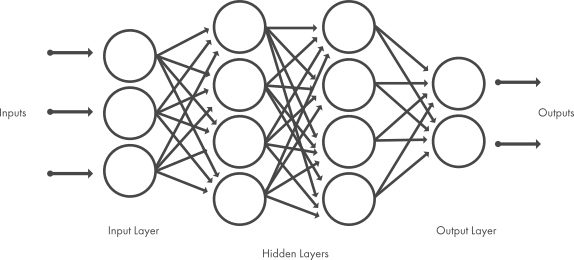
\includegraphics[width=\textwidth]{gambar/deeplearning_layer.png}
    \caption{Contoh \textit{Deep Learning} dengan 4 layer \cite{mathwork_deeplearning}}
    \label{fig: deeplearning_layer}
\end{figure}

% \section{\textit{Transformer}}

% \textit{Transformer} merupakan model \textit{deep learning} yang paling mutakhir saat ini. Tujuan dari \textit{transformer} sendiri sebagai pengembangan dari model rekuren (\textit {Recurrent Neural Network(RNN), Long Short-Term Memory(LSTM)}) ditambah dengan metode \textit{attention span} yang biasanya digunakan untuk melakukan suatu tugas dimana model harus "mengingat" masukan sebelumnya. Model rekuren seperti ini sangat berguna untuk suatu masukan yang bersifat sekuensial, seperti teks atau video sehingga sangat cocok untuk tugas yang memproses banyak teks seperti \textit{Natural Language Understanding (NLU)} atau mesin translasi otomatis \cite{lion_transformer}.

% Namun, kelemahan yang cukup fatal adalah ketidakmampuan model rekuren ini untuk memproses data secara paralel sehingga semakin panjang data yang dimasukkan, maka semakin pula proses yang diperlukan untuk proses \textit{training} maupun saat model sudah berjalan \cite{attention_is_all_you_need}. Ide dasar dari metode \textit{transformer} ini adalah membuang bagian rekuren dari model rekuren yang sudah ada, dan hanya menggunakan bagian \textit{attention span}-nya saja atau dalam metode ini disebut sebagai \textit{self-attention}.

\section{BERT}
BERT merupakan suatu model yang cukup baru dan merupakan singkatan dari \textit{\textbf{B}idirectional \textbf{E}ncode \textbf{R}epresentations from \textbf{T}ransformers}, adalah sebuah model bahasa yang sudah dilakukan proses \textit{pretrained} dengan menggunakan pendekatan \textit{fine-tuning}. BERT merupakan hasil penggabungan antara \textit{bi-directionality} dan \textit{transformer encoder}. \cite{devlin2019bert}

\begin{figure}[h]
    \begin{center}
        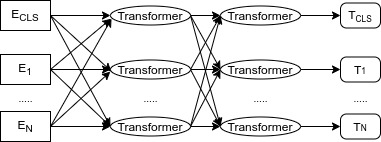
\includegraphics[width= .8\linewidth]{gambar/bert_archi_base.png}
        \caption{pendekatan dua arah BERT}
        \label{fig: bidirectionalBert}
    \end{center}
\end{figure}

Masukan dari BERT dapat berupa teks mentah dengan sedikit melakukan \textit{preprocessing} sebelumnya. Awalnya, BERT akan melakukan \textit{word embedding}, yaitu suatu metode untuk mendapatkan token dari kata yang dimasukkan berdasar pada kamus. Karena proses ini pulalah, terdapat beberapa versi BERT yang khusus untuk bahasa tertentu dan ada juga versi BERT untuk beberapa bahasa sekaligus. Setelah melakukan \textit{word embedding}, BERT akan memasukkan token \texttt{[CLS]}. Token tersebut digunakan sebagai representasi keseluruhan teks dan dapat digunakan sebagai basis dari proses klasifikasi. Selanjutnya, BERT akan membagi kalimat menggunakan token \texttt{[SEP]}. Dari token tersebut akan didapat \textit{segment embeddings} yang berfungsi untuk membedakan antara kalimat A dan kalimat B. \textit{Embedding} yang terakhir adalah berupa \textit{position embedding} yang digunakan untuk menunjukkan posisi kata dalam suatu kalimat. Gambar \ref{fig: bertToken} merupakan gambaran secara garis besar bagaimana BERT memahami suatu input.

\begin{figure}[h!]
    \begin{center}
        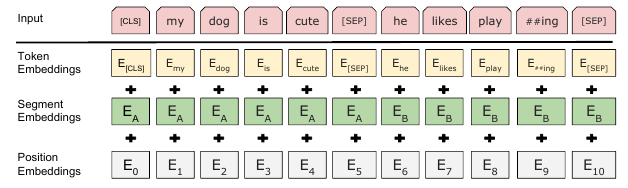
\includegraphics[width= 0.9\linewidth]{gambar/bert.png}
        \caption{Token dalam BERT \cite{devlin2019bert}}
        \label{fig: bertToken}
    \end{center}
\end{figure}

Keluaran dari BERT adalah berupa token - token yang merepresentasikan kalimat tersebut. Nantinya, token - token tersebut dapat digunakan sebagai masukan dari algoritma lain seperti misalnya CNN, maupun menggunakan isi token \texttt{[CLS]} sebagai masukan algoritma klasifikasi seperti \textit{Logistic Regression}.

Keuntungan dari penggunaan BERT adalah apabila dibandingkan dengan \textit{word2vec} yang juga sama - sama merubah kata - kata menjadi vektor atau token adalah, BERT tidak hanya merubah kata - kata tersebut menjadi token saja, namun juga melakukan relasi dan konteks \textit{learning} sehingga token dapat lebih menunjukkan konteks dari kalimat. Sebagai contoh, dalam kalimat "hadiah untuk ibuku sudah dikemas" dan kalimat "acara tersebut dikemas dengan rapi". Kata - kata "dikemas" disini memiliki 2 arti yang berbeda, yang pertama adalah berarti dibungkus, sedangkan yang kedua adalah ditampilkan. Apabila kita menggunakan \textit{word2vec} biasa, kata - kata "dikemas" akan memiliki token yang sama, sedangkan apabila menggunakan BERT, kata tersebut akan memiliki token yang berbeda. \cite{coenen2019visualizing}

Di Indonesia sendiri sudah terdapat beberapa model BERT yang khusus untuk bahasa Indonesia seperti model yang dibuat oleh Cahya dengan menggunakan gabungan dari 522 MB wikipedia Indonesia dan 1GB surat kabar Indonesia \cite{cahya_bert}, dan IndoBERT dengan 12 \textit{layer} dan dilatih menggunakan 31,923 kata dalam bahasa Indonesia \cite{koto2020indolem}. Hal ini kurang lebih sama dengan ukuran BERT-\textit{Base} yang juga memiliki 12 \textit{layer} dan 30,000 kata dalam bahasa Inggris \cite{devlin2019bert}.

\section{Metode Analisa Performa}
Terdapat beberapa metode yang bisa dilakukan untuk mengetahui apakah suatu model memiliki akurasi yang cukup. Penelitian ini menggunakan beberapa formula yang sudah ditentukan seperti \textit{recall, precision, f1-score} dan \textit{confusion matrix}.

\subsection{\textit{Recall}}

\textit{Recall} adalah formula yang harus digunakan ketika kita memiliki data yang tidak seimbang. Berbeda dengan akurasi yang hanya menghitung persentase model memprediksi hasil yang sesuai dengan label secara keseluruhan, \textit{recall} akan menghitung rasio nilai yang diprediksi positif dengan total keseluruhan nilai yang positif \cite{metrics_ml}. Rumus \ref{form:recall} merupakan rumus untuk menghitung \textit{recall}.

\begin{equation}
    Recall = \frac{TP}{TP+FN}
    \label{form:recall}
\end{equation}

\subsection{\textit{Precision}}

Seringnya, kita tidak hanya melihat tingkat akurasi suatu model hanya dengan besaran \textit{recall} maupun tingkat akurasi nya. \textit{Precision} adalah formula untuk menghitung rasio dari prediksi TP (\textit{True Positive}) yang benar dengan keseluruhan prediksi. Apabila prediksi yang dilakukan oleh model kita ternyata memiliki tingkat presisi yang tinggi namun memiliki tingkat \textit{recall} yang rendah, ada kemungkinan model tidak dapat melakukan prediksi pada data yang bersifat negatif \cite{metrics_ml}. Rumus \ref{form:precision} merupakan rumus untuk menghitung nilai dari \textit{precision} suatu model.

\begin{equation}
    Precision = \frac{TP}{TP+FP}
    \label{form:precision}
\end{equation}

Baik \textit{recall} maupun \textit{precision} merupakan nilai yang cukup penting terutama pada data yang tidak seimbang. Terdapat 3 kondisi yang umum terjadi pada saat membandingkan antara \textit{precision} dengan \textit{recall}.

\begin{itemize}
    \item \textit{Recall} tinggi, \textit{Precision} rendah

          Sebagian besar data positif dapat diprediksi dengan benar (\textit{False Negative} yang Rendah), namun hanya ada sebagian kecil data negatif yang diprediksi dengan benar (\textit{True Negative} rendah).

    \item \textit{Recall} rendah, \textit{Precision} tinggi

          Hasil prediksi model memiliki banyak sekali prediksi negatif (\textit{False Negative} tinggi), namun apabila digunakan untuk memprediksi data positif, maka hasil prediksi sebagian besarnya adalah benar (\textit{False Positive} rendah).

    \item \textit{Recall} tinggi, \textit{Precision} tinggi

          Merupakan hasil yang ideal dalam pembuatan model pembelajaran mesin. Disini didapatkan bahwa baik hasil prediksi untuk data positif maupun hasil prediksi untuk data negatif sebagian besarnya adalah benar (\textit{True Positive} dan \textit{True Negative} tinggi).

\end{itemize}

\subsection{\textit{F1-Score}}

\textit{F1-Score} adalah besaran yang berasal dari rata - rata harmonik dari \textit{recall} dan \textit{precision}. Rata  - rata harmonik dipilih karena akan menghasilkan nilai rata - rata yang lebih rendah dalam kondisi tidak seimbang apabila dibandingkan dengan rata - rata aritmatis biasa. Dengan rata - rata seperti itu, suatu model dapat menjadi lebih rentan terhadap bias dan memudahkan pada saat pembuatan model \cite{metrics_ml}. Rumus \ref{form: f1-score} merupakan rumus untuk menghitung f1-score.

\begin{equation}
    \label{form: f1-score}
    F1-Score = 2 \times \frac{\textit{Recall} \times \textit{Precision}}{\textit{Recall} + \textit{Precision}}
\end{equation}

\subsection{\textit{Confusion Matrix}}

\textit{Confusion Matrix} adalah tabel kesimpulan yang berisi jumlah prediksi baik yang benar maupun yang salah dan nilai label baik yang benar maupun salah. Biasanya tabel jenis ini digunakan untuk tugas yang bersifat klasifikasi dan berfungsi untuk memvisualisasi bagaimana suatu performa model dalam suatu dataset.

\begin{table}
    \caption{Contoh \textit{Confusion Matrix}}
    \label{tab:cth_confusion_mtrx}
    \centering
    \begin{tabular}{|l|l|l|l|l}
        \cline{1-4}
        \multicolumn{2}{|l|}{\multirow{2}{*}{}} & \multicolumn{2}{l|}{\textbf{Aktual}} &                \\ \cline{3-4}
        \multicolumn{2}{|l|}{}                  & Positif                              & Negatif &      \\ \cline{1-4}
        \multirow{2}{*}{\textbf{Prediksi}}      & Positif                              & TP      & FP & \\ \cline{2-4}
                                                & Negatif                              & TN      & FN & \\ \cline{1-4}
    \end{tabular}
\end{table}

Tabel \ref{tab:cth_confusion_mtrx} adalah contoh tabel \textit{confussion matrix} untuk prediksi dengan 2 label. Apabila melihat pada tabel tersebut, dapat terlihat bahwa jumlah prediksi dipecah menjadi masing - masing kelas. Diharapkan dengan dipecah menjadi beberapa kelas seperti itu, akan membuat proses pengujian lebih mudah karena akan lebih mudah melihat pada saat model memprediksi jenis data apa yang masih memiliki tingkat akurasi yang kurang bagus. Terdapat beberapa hal yang harus diketahui untuk dapat memahami sebuah tabel \textit{confussion matrix}, yaitu :

\begin{itemize}[nolistsep]
    \item Positif (P)

          Berisi data yang bernilai positif, baik data tersebut beasal dari hasil prediksi maupun data aktual yang didapat dari dataset.

    \item Negatif (N)

          Berisi data yang bernilai negatif, baik data tersebut berasal dari hasil prediksi maupun data aktual yang didapat dari dataset.

    \item \textit{True Positive} (TP)

          Suatu kondisi dimana baik hasil prediksi maupun data aktual sama - sama bernilai positif. Semakin tinggi nilai dari TP, semakin akurat pulalah model yang sudah dibuat.

    \item \textit{False Positive} (FP)

          Suatu kondisi dimana hasil prediksi adalah positif, namun pada data aktual bernilai negatif. Biasanya, semakin tinggi nilai dari FP ini, maka model semakin memilki kecenderungan untuk mengeluarkan nilai positif dibanding negatif atau terjadinya bias pada model.

    \item \textit{True Negative} (TN)

          Suatu kondisi dimana hasil prediksi adalah negatif, namun pada data aktual bernilai positif. Biasanya, semakin tinggi nilai dari TN ini, maka model semakin memiliki kecenderungan untuk mengeluarkan nilai negatif dibanding positif.

    \item \textit{False Negative} (FN)

          Suatu kondisi dimana hasil prediksi dan data aktual bernilai negatif. Semakin tinggi nilai FN berarti semakin akurat model yang sudah dibuat.

\end{itemize}
